\chapter{Introducción}
\label{cap:Introduccion}
Actualmente la demanda energética en el planeta no deja de crecer, y por tanto deben llevarse a cabo medidas para reducir el consumo elevado de energía, lo que se conoce como eficiencia energética. La eficiencia energética~\cite{GarSa12} se refiere al empleo de medios de optimización en la producción y aprovechamiento de la energía, con el objetivo de proteger el medio ambiente. Esto ha pasado a ser una necesidad debido a que las emisiones de $ CO_{2} $ van en aumento y el cambio climático es un hecho.\\

Por otro lado, puesto que las fuentes de energía fósil y nuclear son finitas, podría llegar el día en el que no se pueda satisfacer la demanda energética, salvo que se apueste por los métodos alternativos de obtención de energía. Es aquí donde entran en juego las energías renovables. Una de ellas es la energía solar~\cite{Perp12}, que permite el aprovechamiento de la radiación electromagnética del sol. Resulta interesante su estudio, debido a que es tan abundante que se considera inagotable: la cantidad de energía que el Sol vierte diariamente sobre la Tierra es diez mil veces mayor que la consumida al día en todo el planeta. Finalmente, además de ser una energía inagotable, es una energía limpia, una muy buena alternativa a los combustibles fósiles o a la energía nuclear. \\

Teniendo en cuenta estos dos antecedentes, existe una motivación a la hora de apostar por medios de extracción de energía renovables y por la eficiencia energética. Actualmente la mayoría de hogares consumen energía de manera exclusiva de la red eléctrica, lo que significa que importan la totalidad de la energía que su hogar demanda a una compañía eléctrica, a un precio establecido \gls{PVPC}~\cite{Ree14} (Precio voluntario al pequeño consumidor) que representa el precio máximo de referencia que pueden contratar los consumidores con hasta 10 Kwh de potencia disponible. Hoy en día existen un gran número de fuentes de extracción de energía cuyos precios y potencias generadas varían a lo largo del tiempo, e incluso del día. Estos cambios son dependientes de un gran número de factores. Sería interesante poder reducir la cantidad de energía que se obtiene de la red eléctrica en las horas pico (horas de máximo consumo donde el \gls{PVPC} suele alcanzar el valor alto) y obtenerla de otra fuente cuyo precio sea menor, para así obtener un promedio mucho mas barato que con una única fuente de energía. Esto puede lograrse incorporando nuevas fuentes, como puede ser la instalación de módulos fotovoltaicos. Este procedimiento está regulado, pues en el año 2015 mediante el Real Decreto 900/2015~\cite{Boe15} se establecieron unas condiciones para la instalación de placas fotovoltaicas, lo que se conoce coloquialmente como el impuesto al sol. Por suerte, a las potencias contratadas no superiores a 10 Kwh no aplica este impuesto, así que no supone un problema en el caso de un hogar de tamaño normal.\\

En este \gls{TFG} se ha decidido enfocar la base de conocimientos adquiridos por el alumno durante el Grado en Ingeniería Informática para plantear una solución a la problemática anterior. Se propone la creación de un sistema inteligente para que la gestión de energía en hogares se realice de una manera óptima y eficiente. Para ello será necesaria la instalación de módulos fotovoltaicos y una batería. Tras esto un hogar dispondría de varias fuentes de energía, lo que permite obtener la energía demandada de la fuente más barata en cada momento, como se comentó antes. Esto va a ser posible modelando la instalación como un problema de satisfacción de restricciones (\gls{PSR}) que contará con un conjunto de variables, que representan las fuentes de generación y consumo de energía implicadas. Los valores de estas variables representan la cantidad de energía obtenida de cada fuente y serán condicionados por unas restricciones van a estar determinadas por la configuración existente en el hogar y se adecuarán a las propiedades físicas que tiene la generación y consumo de energía así como a la condición climática en cada momento. La combinación óptima de valores para estas variables representa la solución buscada, que tiene como consecuencia un ahorro en el coste energético. En la Figura~\ref{fig:abstract} se muestra una representación del sistema propuesto donde se identifican desde un alto nivel de abstracción los elementos generadores de energía y los elementos consumidores.\\
\begin{figure}[!h]
	\centering
	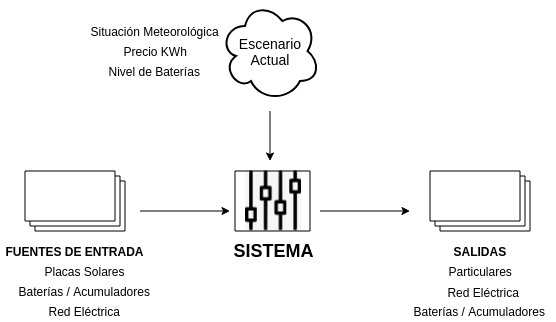
\includegraphics[width=10cm]{figs/Abstract.png}
	\caption{Representación del sistema}
        \label{fig:abstract}
\end{figure}


\section{Estructura del TFG}
Este documento está formado por los capítulos expuestos a continuación
\begin{description}
\item \textbf{~\ref{cap:Introduccion}. Introducción}\\
  Se muestra la problemática inicial, se plantea e introduce este \gls{TFG} como solución y se muestra un esquema abstracto del sistema propuesto.
\item \textbf{~\ref{cap:Objetivo}. Objetivos}\\
  Se plantean y definen tanto el objetivo principal como los objetivos parciales a desarrollar.
\item \textbf{~\ref{cap:Antecedentes}. Antecedentes}\\
  Se muestra el estado del arte y se definen los conceptos de computación mas importantes que se emplean en este proyecto.
\item \textbf{~\ref{cap:Metodologia}. Metodología}\\
  Se muestra y define la metodología de proyecto empleada. Se habla acerca de como ha sido adaptada a este caso particular y se describen las tecnologías y herramientas utilizadas.
\item \textbf{~\ref{cap:Resultados}. Resultados}\\
  Se describen los resultados obtenidos a lo largo del desarrollo del \gls{TFG} desde el inicio hasta el final, siguiendo la metodología definida, problemas encontrados y soluciones empleadas.
\item \textbf{~\ref{cap:Conclusiones}. Conclusiones}\\
  Se habla acerca de las conclusiones e ideas obtenidas tras finalizar el proyecto y se plantean posibles ampliaciones y trabajo futuro.
\item \textbf{Anexo~\ref{cap:AnexoA}. Caso de optimización}\\
  Se puede consultar el resumen de una simulación para el día 11/04/2019.
\item \textbf{Anexo~\ref{cap:AnexoB}. \textit{Tests} del proyecto}\\
  Se explica el framework de \textit{tests} usado para realizar los casos de prueba del proyecto software. Esto es necesario pues garantiza tolerancia a fallos y demuestra la funcionalidad del sistema.
\end{description}
